\documentclass{article}

% --- Required Packages ---
\usepackage[a4paper, margin=0in]{geometry}
\usepackage{fontspec}
\usepackage[svgnames]{xcolor}
\usepackage{graphicx}
\usepackage{tikz}
\usetikzlibrary{positioning}
\usepackage{hyperref}
\hypersetup{
    colorlinks=true,
    linkcolor=blue,
    filecolor=magenta,      
    urlcolor=cyan,
    pdftitle={Krider's Field Guide}, % Corrected document title
    pdfpagemode=FullScreen,
    }

% --- COLOR PALETTE ---
\definecolor{PaperColor}{HTML}{FDF5E6}
\definecolor{TextColor}{HTML}{36454F}
\definecolor{KriderYellow}{HTML}{FDF5E6}
\definecolor{KriderGreen}{HTML}{5E7756}
\definecolor{KriderDarkText}{HTML}{36454F}

% --- Document-wide Settings ---
\setmainfont{Roboto}[
    UprightFont = *,
    BoldFont = * Bold,
    ItalicFont = * Italic
]
\pagenumbering{gobble}

% --- Document Body ---
\begin{document}
\pagestyle{empty}

%---------------------------------------------------
% PAGE 1: Krider's Field Guide Cover (Corrected Layout)
%---------------------------------------------------
\begin{tikzpicture}[remember picture, overlay]
    \coordinate (C) at (current page.center);

    % --- Background ---
    \fill[KriderYellow] (current page.south west) rectangle (current page.south east);

    % --- Header Block ---
    \node[KriderDarkText, anchor=north west, align=left] at (current page.north west) [xshift=1.5cm, yshift=-1.5cm] {
        \normalfont \fontsize{10}{12}\selectfont Powered by \{data\}syntax
    };
    
    % --- Main Title (Above Image) ---
    \node[KriderDarkText, anchor=center, text centered] at (current page.north) [yshift=-3cm] {
        \bfseries \fontsize{50}{66}\selectfont Krider's  Field Guide
    };
    
    % --- Subheadings ---
    \node[KriderDarkText, anchor=center] at (current page.north) [yshift=-5cm] {
        \normalfont\itshape \fontsize{16}{20}\selectfont Continuing a Legacy of Horticultural Excellence Since 1906 
    };

    % --- Main Image (Resized and placed below the title) ---
    \node[anchor=center] at ([yshift=.8cm]C) {
        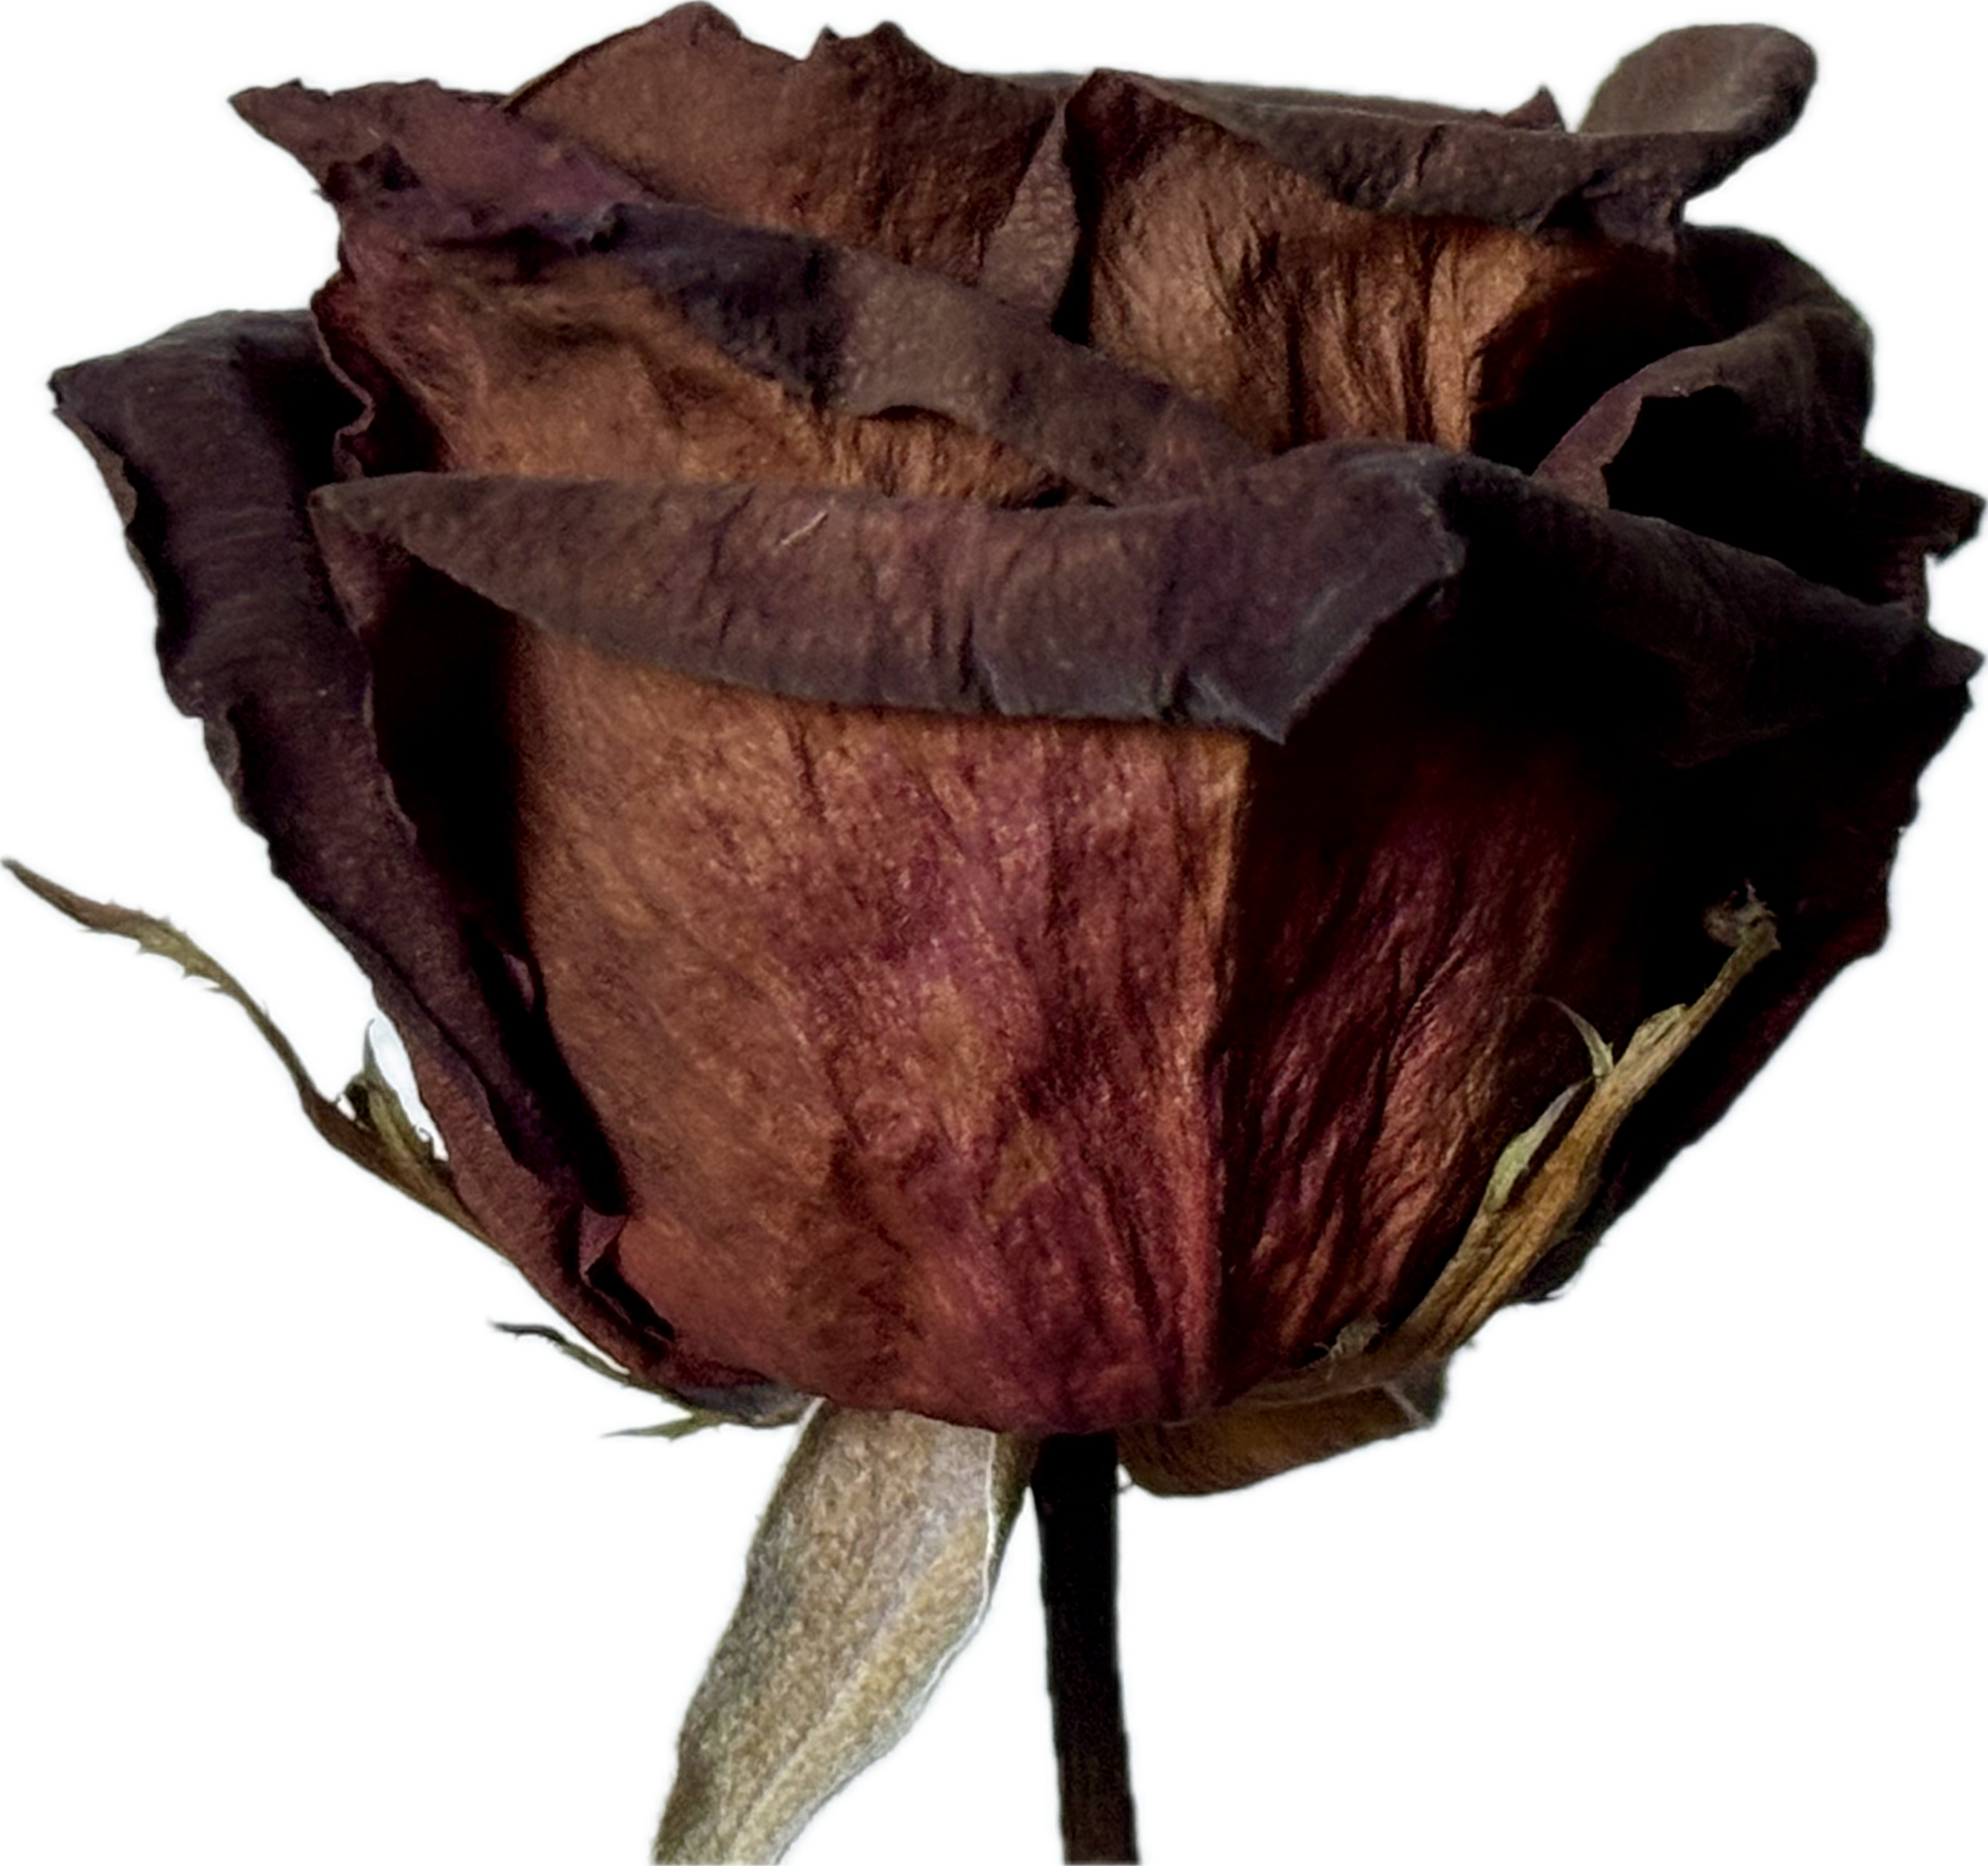
\includegraphics[width=16.5cm]{coverRose.png}
    };
    
    % --- Bottom Product Box (with green background) ---
    \node[fill=KriderGreen, text=white, anchor=south, minimum width=\paperwidth-2cm, inner sep=15pt, outer sep=0, rounded corners=3pt] at (current page.south) [yshift=3.8cm] {
        \begin{minipage}{0.9\textwidth}
            \bfseries \fontsize{18}{20}\selectfont Tea rose (Rosa × odorata (Andrews) Sweet) \\[3mm]
            \normalfont \fontsize{14}{15}\selectfont (Illustrated Above). Roses have so many uses. A dried rose, with its preserved form, can be just as impactful as a live one. Symbolizing everything from eternal love to memory and even the mysterious beauty of decay, making it a perfect emblem for the Halloween season.\\
            To create your own, simply hang them upside down in a cool, dark, and dry place for two to three weeks. This simple act of preservation allows them to be appreciated long after the bloom has faded.

        \end{minipage}
    };
    
    % --- Krider Logo Footer (Bottom Left) ---
    \node[anchor=south west, align=left, text width=4in] at (current page.south west) [xshift=1.5cm, yshift=1.5cm] {
        \bfseries\itshape \fontsize{24}{24}\selectfont Krider's Field Guide \\
        \itshape\bfseries \fontsize{10}{12}\selectfont Week 44 - Fall - 2025 \\
        \normalfont\itshape \fontsize{9}{11}\selectfont Guide: 003
    };
    
    % --- Page Footer ---
    \node[KriderDarkText, anchor=center] at (current page.south) [yshift=20] {
        \fontsize{12}{14}\itshape Page 1 of 3
    };
\end{tikzpicture}

\newpage

%---------------------------------------------------
% PAGE 2: Professional 2x2 Rose Grid Page
%---------------------------------------------------
\begin{tikzpicture}[remember picture, overlay]
    \fill[KriderYellow] (current page.south west) rectangle (current page.north east);
    \coordinate (C) at (current page.center);

    % --- Main Title ---
    \node[KriderDarkText, anchor=north, text width=0.9\paperwidth, align=center] at (current page.north) [yshift=-3cm] {
        \bfseries\fontsize{36}{40}\selectfont 
    };

    % --- Define a style for each content block for consistency ---
    \tikzset{rose_block/.style={text width=8cm, align=center}}

    % --- Top Left Rose: Daisy ---
    \node[rose_block] at ([xshift=-5cm, yshift=6.5cm]C) {
        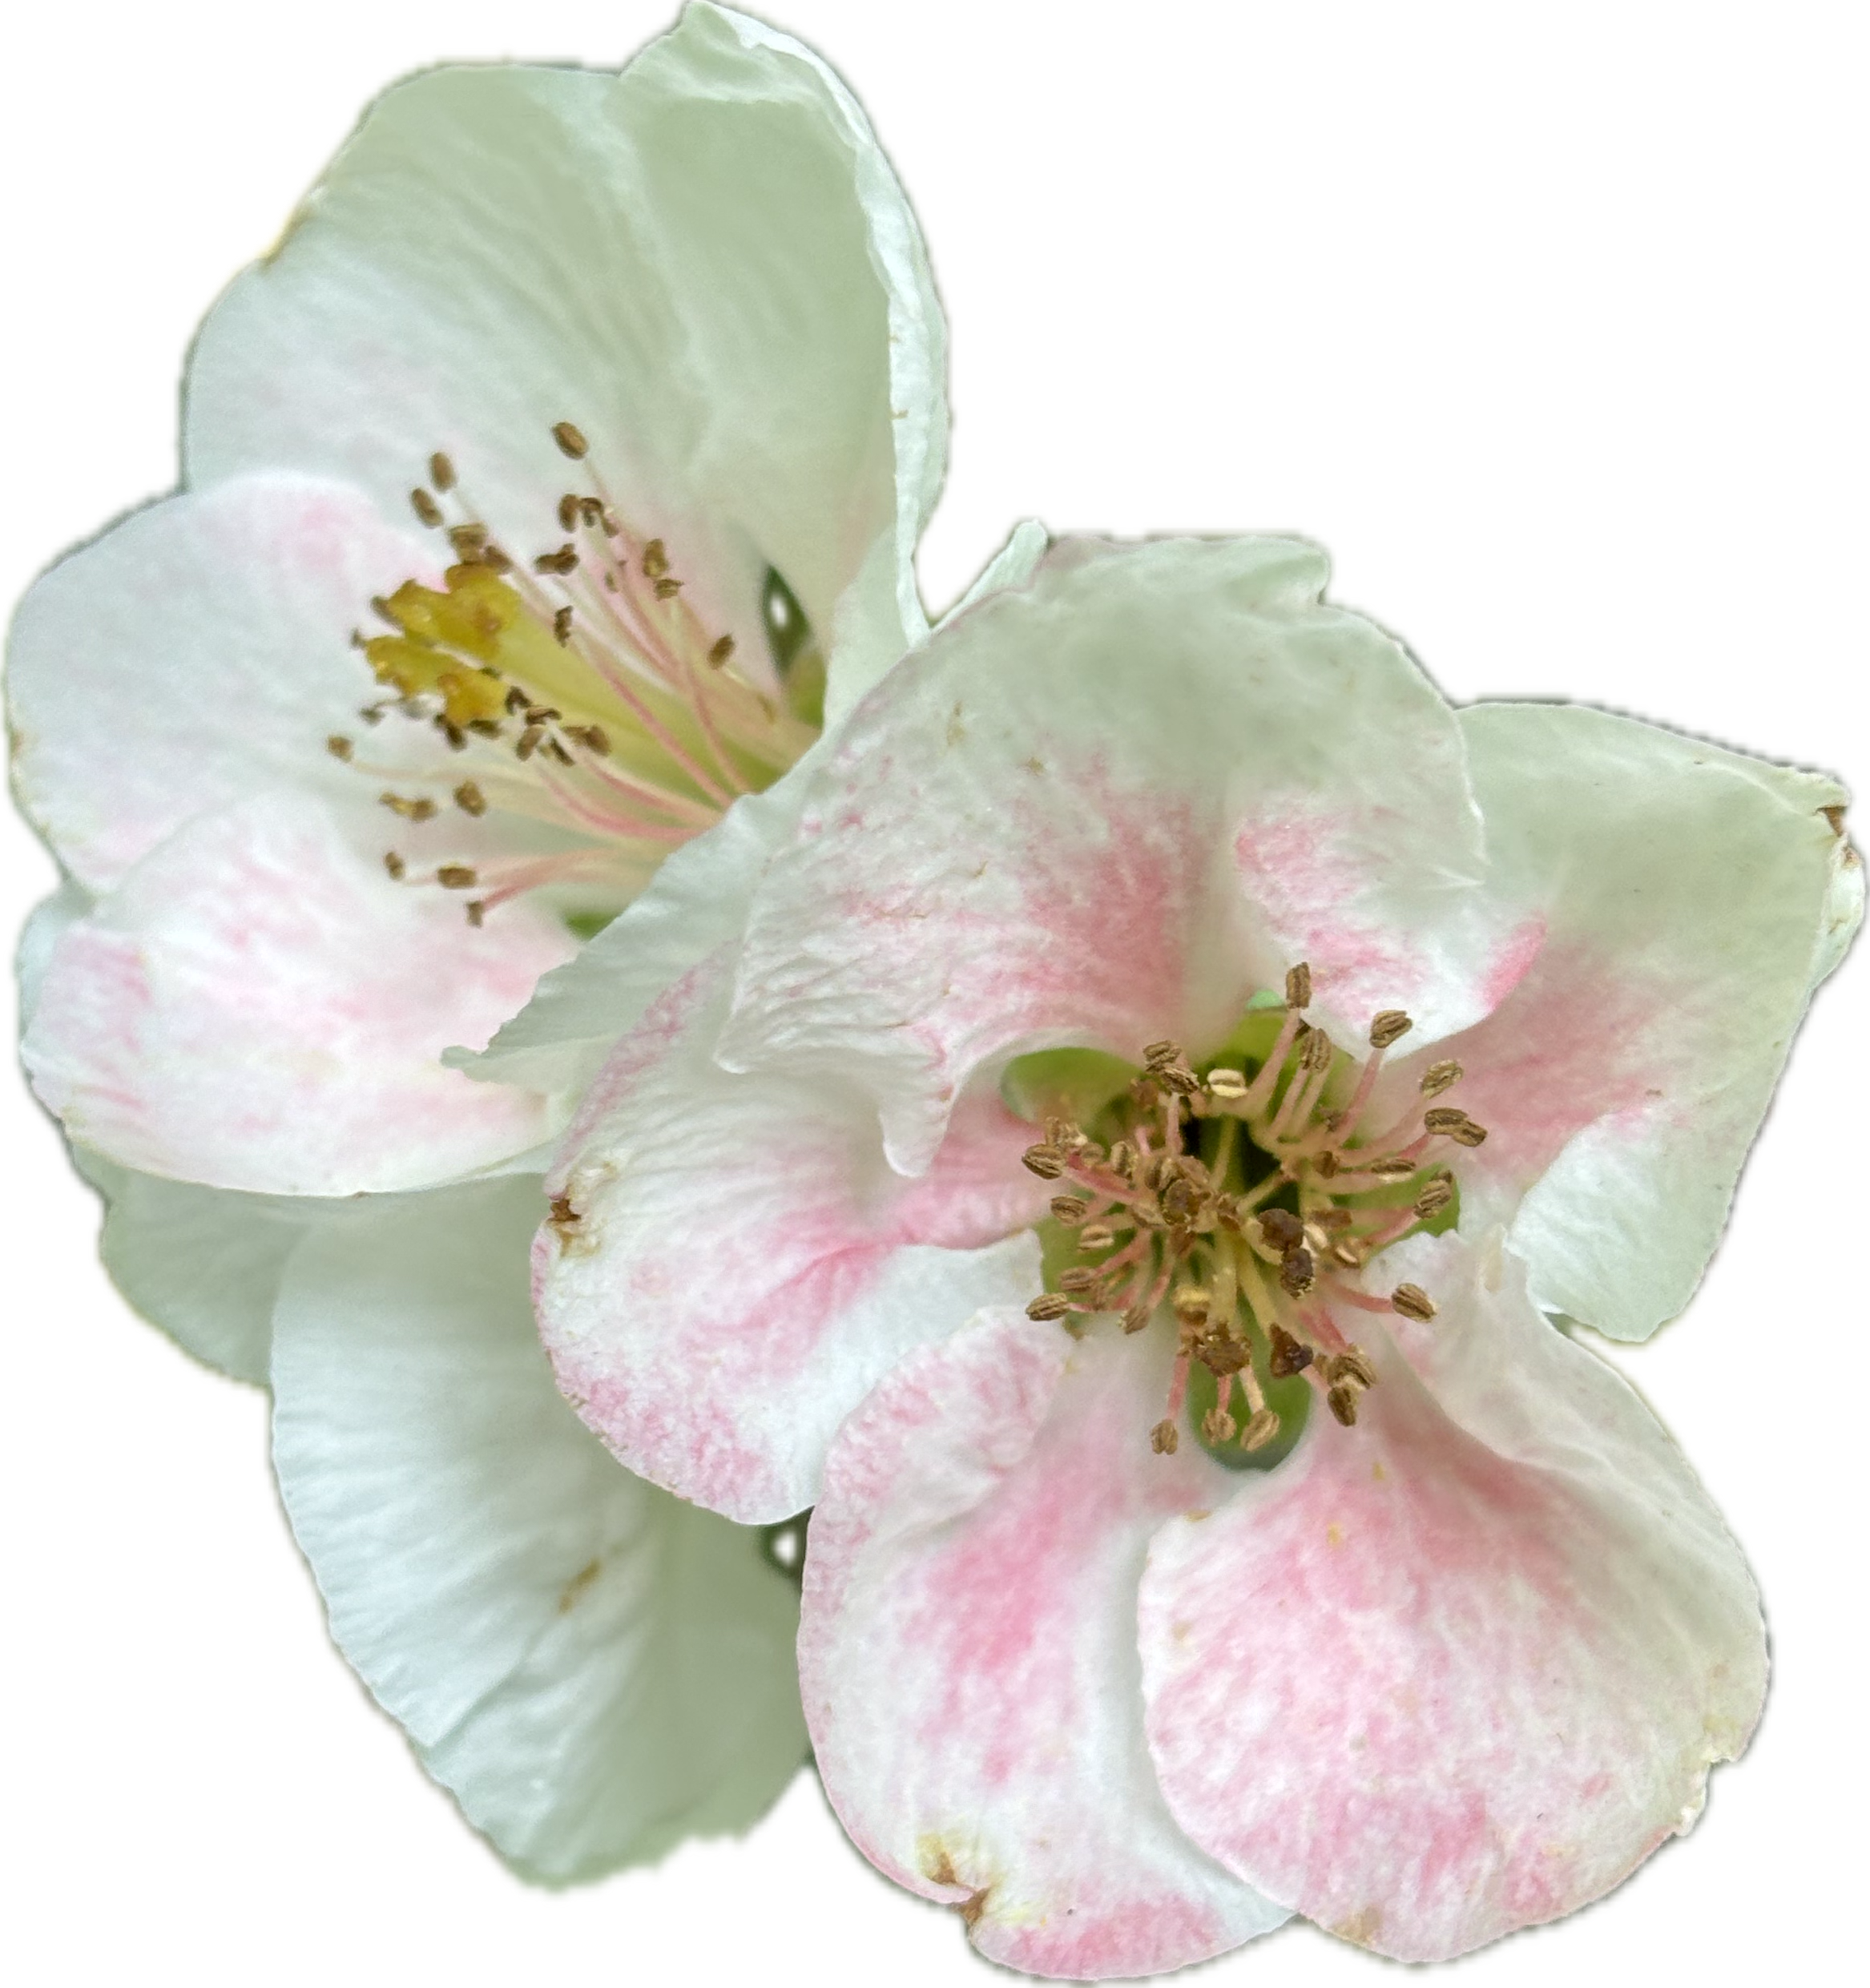
\includegraphics[width=7cm]{flower1.png} \\
        \vspace{5mm}
        \bfseries\fontsize{16}{18}\selectfont Sweet crab apple \\
        \normalfont\itshape\fontsize{11}{13}\selectfont(Malus coronaria (L.) Mill.) \\
        \normalfont\fontsize{12}{13}\selectfont This North American native is a small tree that produces fragrant, pink and white flowers in the spring. Its fruits are small and tart but can be used to make preserves and cider. \\
        
    };

    % --- Top Right Rose: Buccaneer ---
    \node[rose_block] at ([xshift=5cm, yshift=6.5cm]C) {
        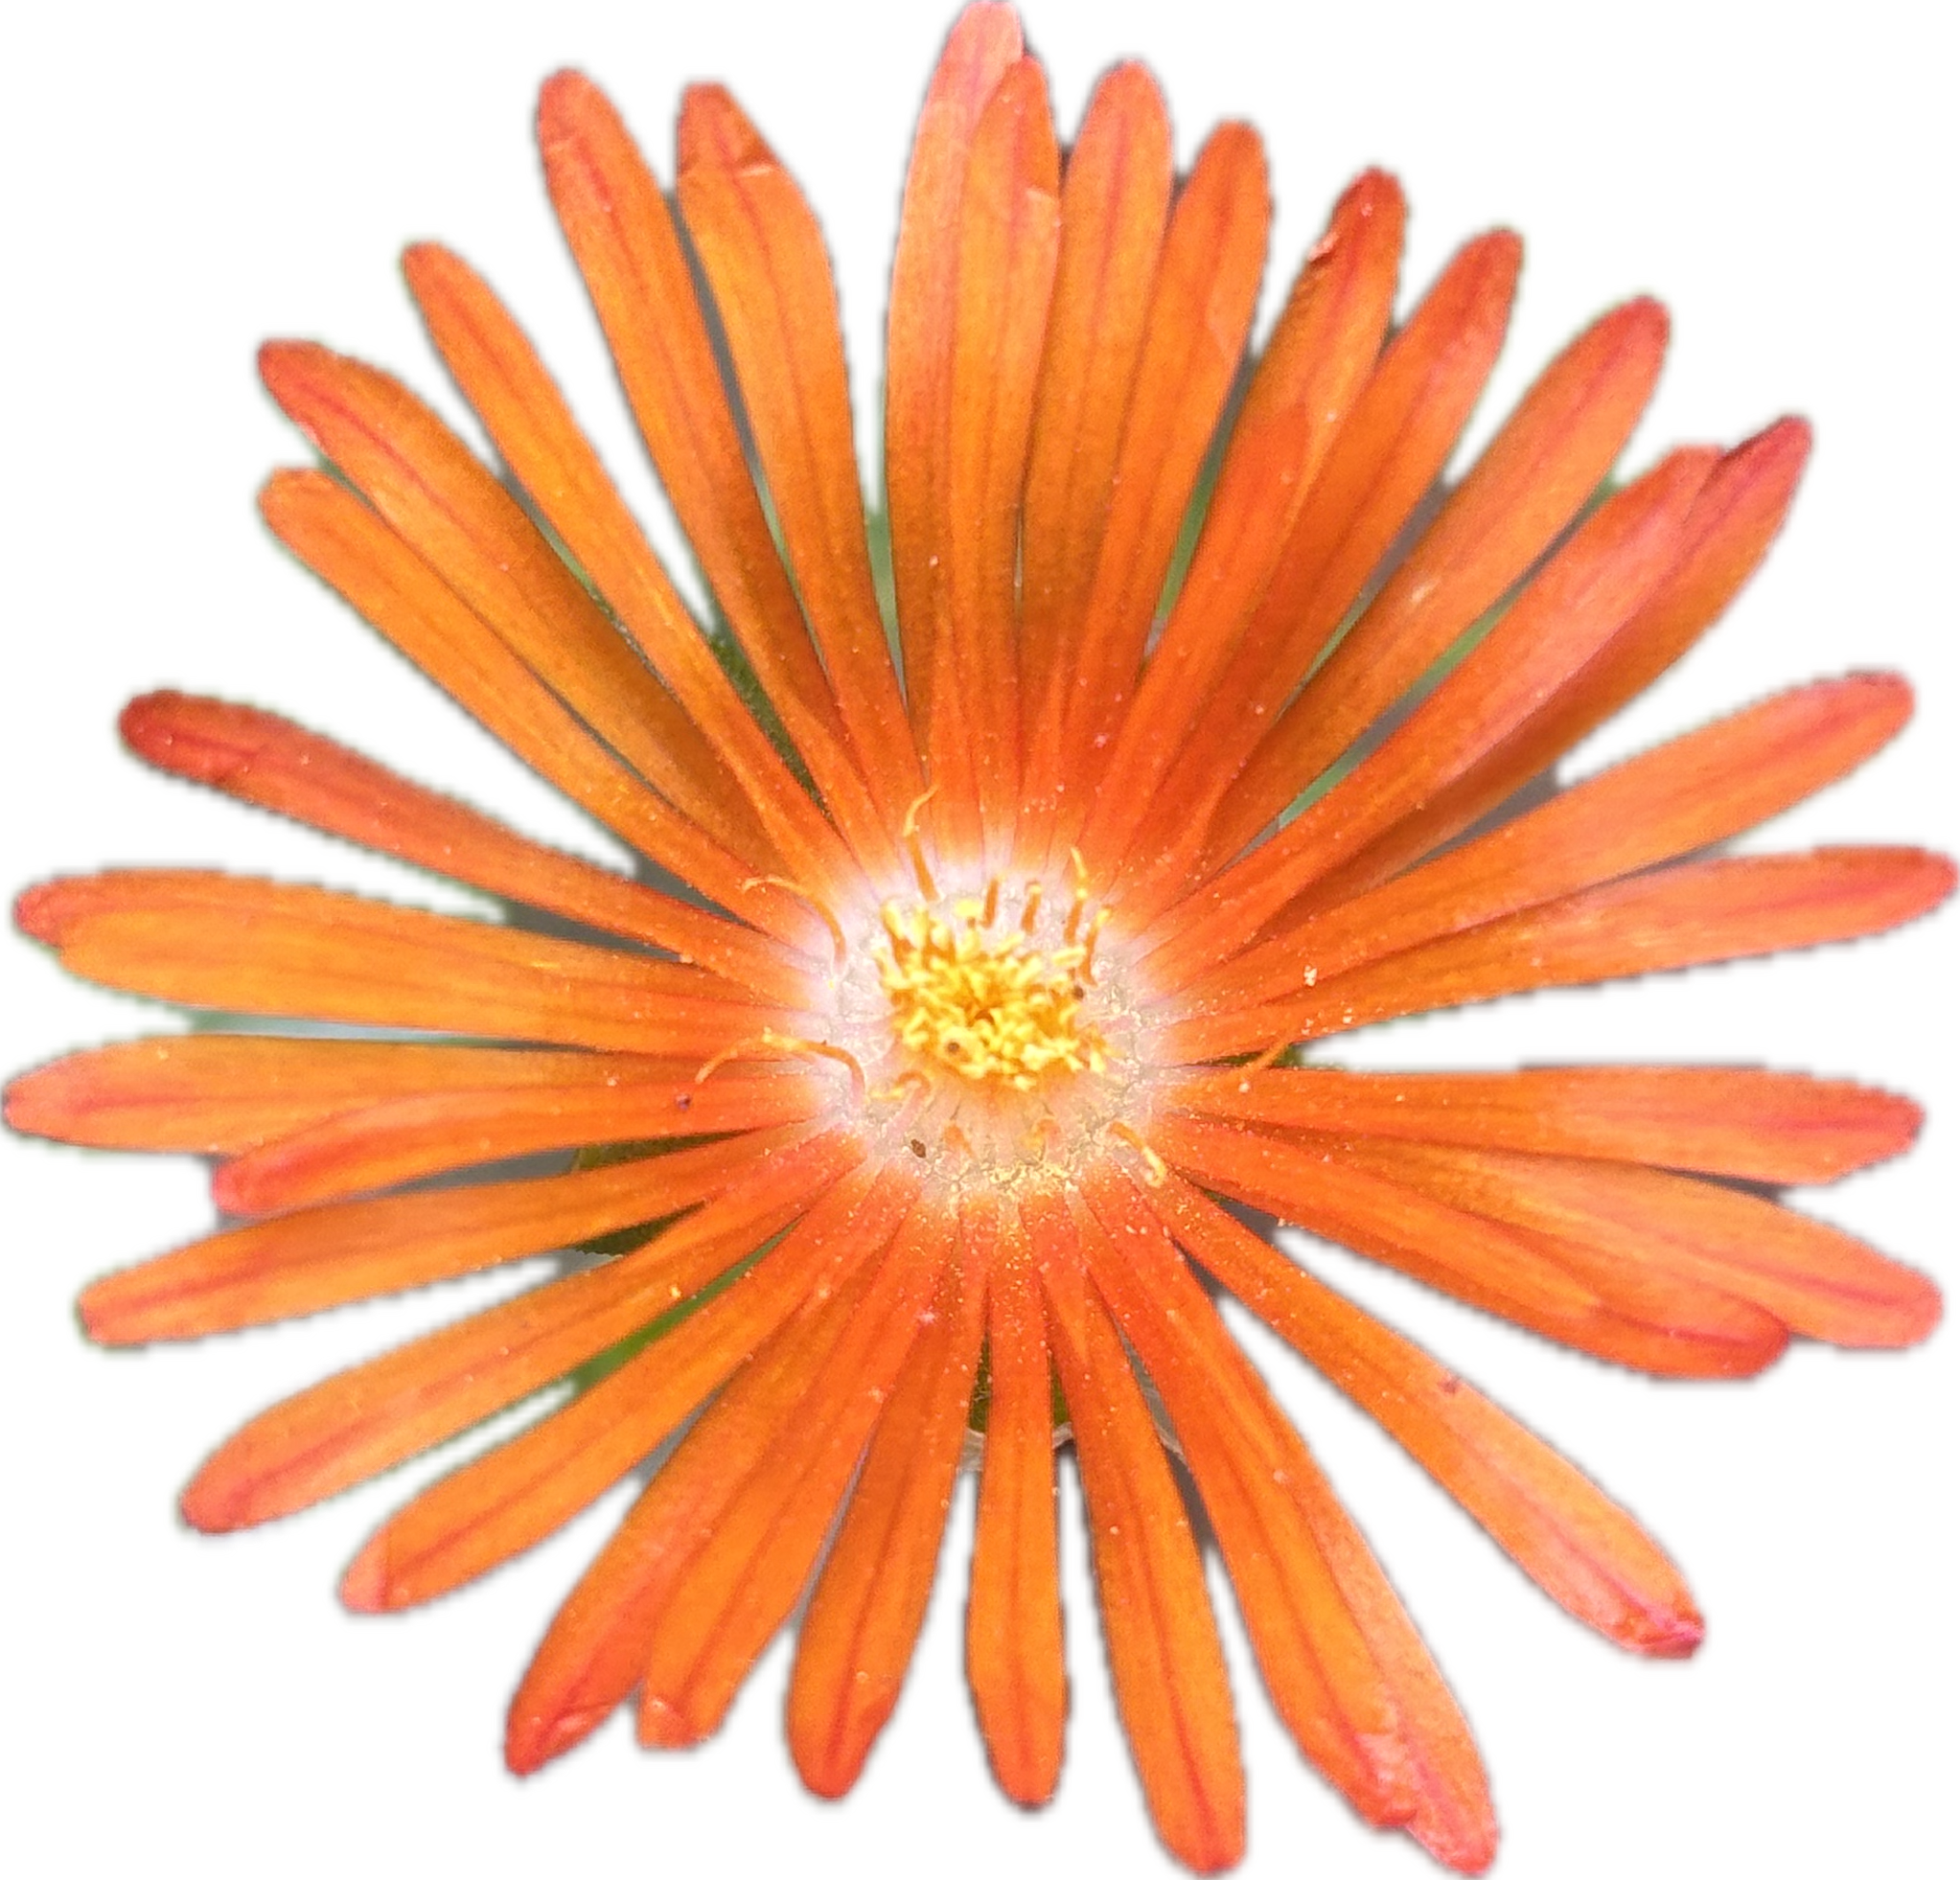
\includegraphics[width=7cm]{flower2.png} \\
        \vspace{5mm}
        \bfseries\fontsize{16}{18}\selectfont Coppery vygie \\
        \normalfont\itshape\fontsize{11}{13}\selectfont (Malephora crocea (Jacq.) Schwantes) \\
        \normalfont\fontsize{12}{13}\selectfont This hardy, succulent ground cover is known for its glistening coppery-orange flowers that open in bright sunlight. It is a drought-tolerant plant that thrives in dry areas and will rot if overwatered. \\
    };

    % --- Bottom Left Rose: Roundelay ---
    \node[rose_block] at ([xshift=-5cm, yshift=-5.5cm]C) {
        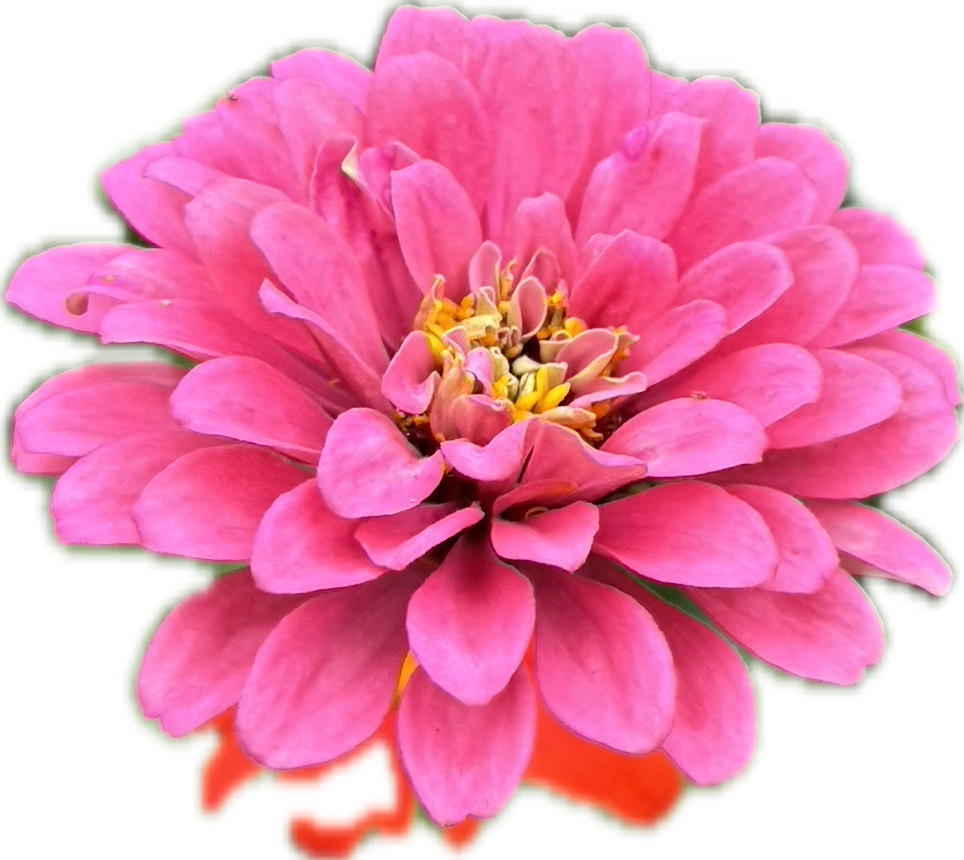
\includegraphics[width=7cm]{flower3.png} \\
        \vspace{5mm}
        \bfseries\fontsize{16}{18}\selectfont Peruvian zinnia \\
        \normalfont\itshape\fontsize{11}{13}\selectfont (Zinnia peruviana (L.) L.) \\
        \normalfont\fontsize{12}{13}\selectfont Native to the Americas, this annual wildflower is recognized by its vibrant, daisy-like flowers in shades of red, orange, and yellow. It is a fast-growing plant that attracts pollinators like bees and butterflies. \\
    };

    % --- Bottom Right Rose: Montezuma ---
    \node[rose_block] at ([xshift=5cm, yshift=-5.5cm]C) {
        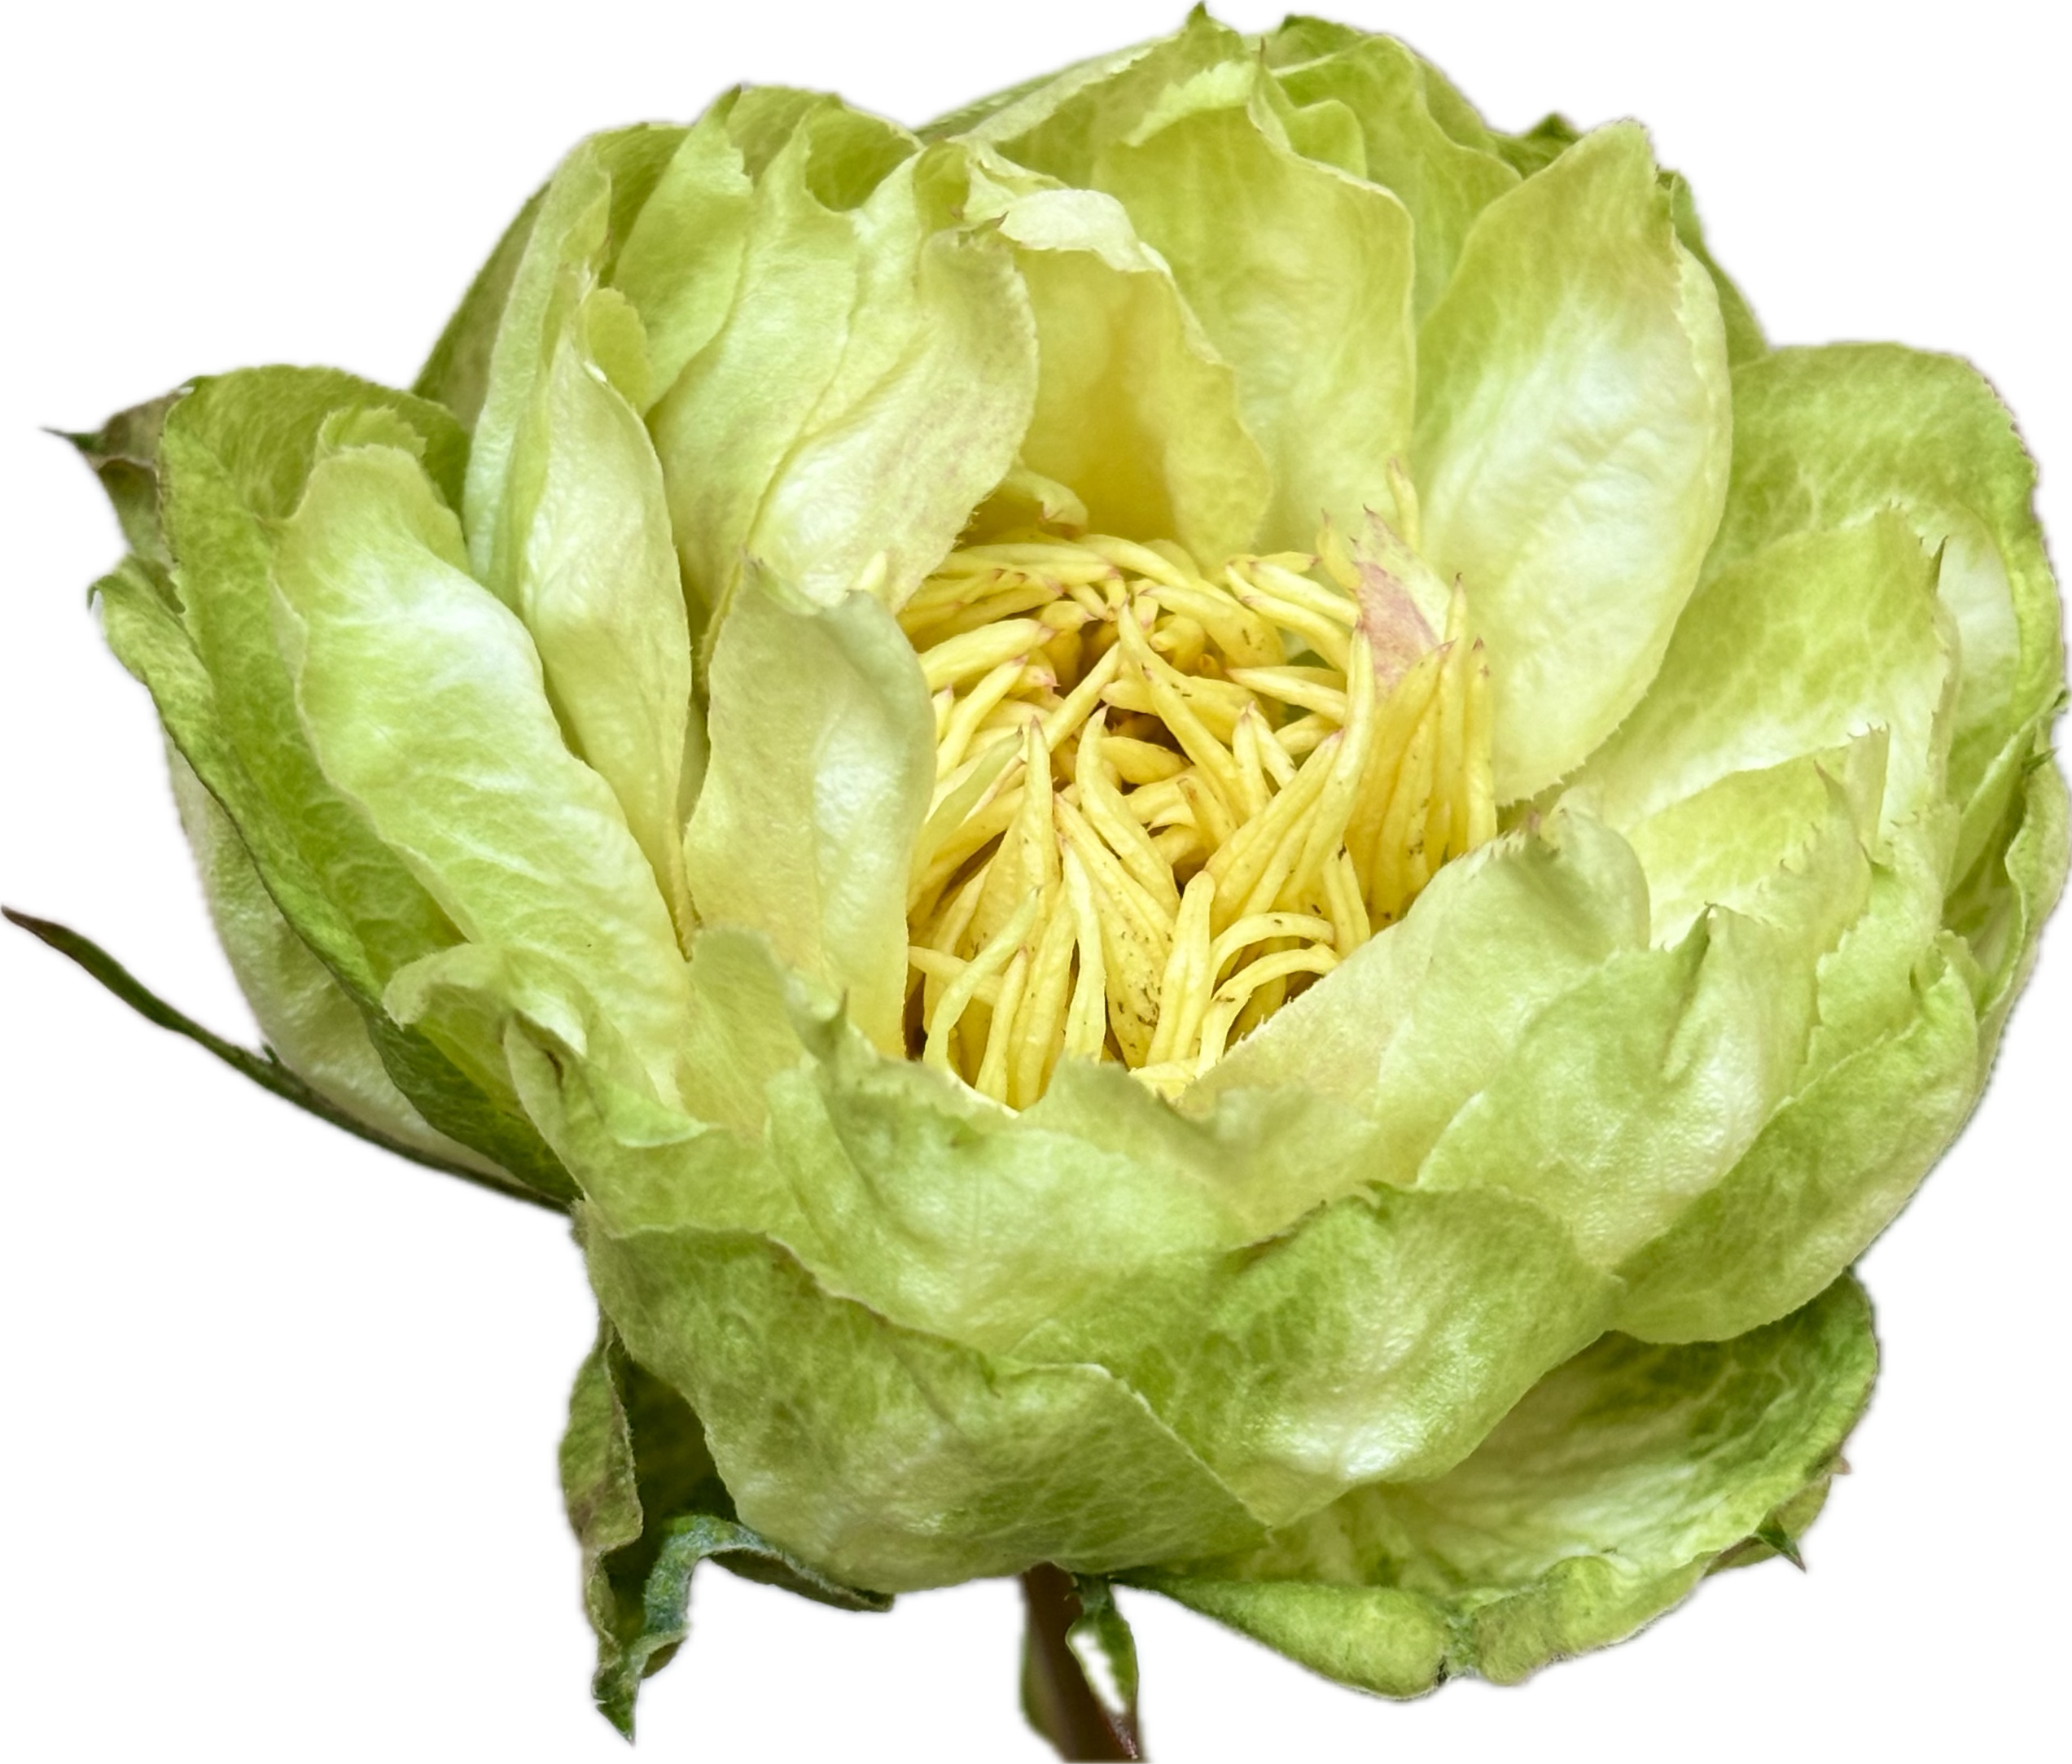
\includegraphics[width=7cm]{flower4.png} \\
        \vspace{5mm}
        \bfseries\fontsize{16}{18}\selectfont Veggie Rose \\
        \normalfont\itshape\fontsize{11}{13}\selectfont (Rosaceae) \\
        \normalfont\fontsize{12}{13}\selectfont Also known as the Green Rose, this unique variety is a sport of the China Rose and is prized for its unusual green blooms. Instead of petals, the 'Viridiflora' has layered, leaf-like sepals and is a true curiosity in the rose world. \\
    };

    % --- Page Footer ---
    \node[KriderDarkText, anchor=center] at (current page.south) [yshift=50] {
        \fontsize{12}{14}\itshape Page 2 of 3
    };
\end{tikzpicture}

\newpage

%---------------------------------------------------
% PAGE 3: CITATION PAGE (Themed)
%---------------------------------------------------
\begin{tikzpicture}[remember picture, overlay]
    \fill[KriderYellow] (current page.south west) rectangle (current page.north east);
    
    % --- Main Title ---
    \node[KriderDarkText, anchor=center] at (current page.center) [yshift=250] {
        \fontsize{32}{36}\bfseries Project Source \& Collaboration
    };
    
    % --- Explanatory Text ---
    \node[KriderDarkText, anchor=north, text width=0.7\paperwidth, align=center] at (current page.center) [yshift=180] {
        \fontsize{14}{22}\selectfont
        This document was written in \LaTeX. The complete source code, image assets, and project history are available on GitHub. Suggestions, and flower requests are welcome!.
    };

    % --- GitHub Logo and Link ---
    \node[anchor=center] at (current page.center) [yshift=-20] {
        \href{https://github.com/Data-Syntax/KridersFieldGuide}{
\includegraphics[height=5cm]{github-mark.png}}
    };
    
    \node[KriderDarkText, anchor=center] at (current page.center) [yshift=-100] {
        \fontsize{14}{18}\selectfont\url{https://github.com/Data-Syntax/KridersFieldGuide}
    };
    
    % --- Page Footer ---
    \node[KriderDarkText, anchor=center] at (current page.south) [yshift=50] {
        \fontsize{12}{14}\itshape Page 3 of 3
    };
\end{tikzpicture}

\end{document}